\documentclass{article}
\usepackage{fancyhdr}
\usepackage{amsthm}
\usepackage{etoolbox}
\usepackage{verbatim}
\usepackage{enumerate}
\usepackage{amsmath}
\usepackage{algorithmicx}
\usepackage{algorithm}
\usepackage{algpseudocode}
\usepackage{amssymb}
\usepackage{tikz}
	
\pagestyle{fancy}
\title{Chapter 19}
\author{Michelle Bodnar, Andrew Lohr}

\newcounter{curnum}
\setcounter{curnum}{0}

\newtheorem{th1}{Exercise} 
\newcommand{\calH}{\mathcal{H}}
\newcommand{\calX}{\mathcal{X}}
\newcommand{\calA}{\mathcal{A}}
\newcommand{\calY}{\mathcal{Y}}

\begin{document}
\maketitle


\noindent\textbf{Exercise 19.2-1}\\
Frst, we take the subtrees rooted at 24, 17, and 23 and add them to the root list. Then, we set H.min to 18. Then, we run consolidate. First this has its degree 2 set to the subtree rooted at 18. Then the degee 1 is the subtree rooted at 38. Then, we get a repeadted subtree of degree 2 when we consider the one rooted at 24. So, we make it a subheap by placing the 24 node under 18. Then, we consider the heap rooted at 17. This is a repeat for heaps of degree 1, so we place the heap rooted at 38 below 17. Lastly we consider the heap rooted at 23, and then we have that all the different heaps have distinct degrees and are done, setting H.min to the smallest, that is, the one rooted at 17.

The three heaps that we end up with in our root list are:

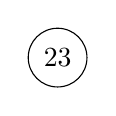
\begin{tikzpicture}[level/.style={sibling distance=30mm/#1}]
\node [circle,draw] (a){23}
;
\end{tikzpicture}

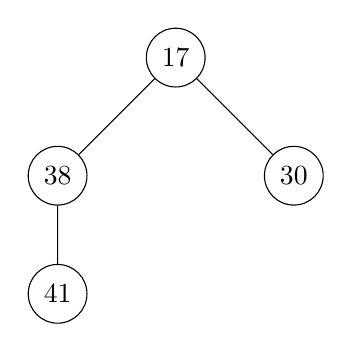
\begin{tikzpicture}[level/.style={sibling distance=30mm/#1}]
\node [circle,draw] (a){17}
  child {
  node [circle,draw] (b) {38}
  child{
  node [circle,draw] (c) {41}
  }
  }
  child {
  node [circle,draw] (d) {30}
  }
;
\end{tikzpicture}

and

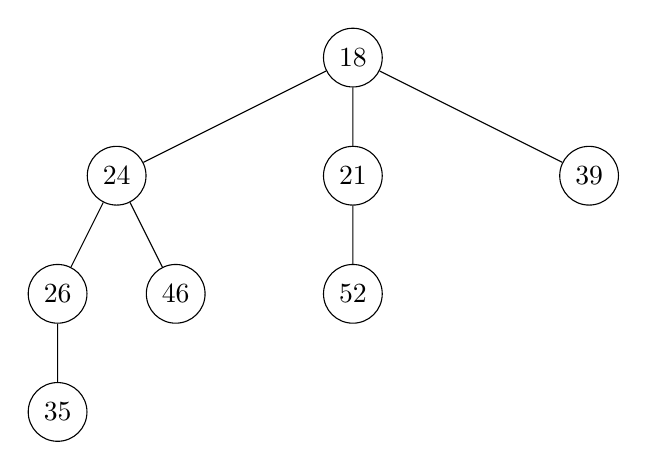
\begin{tikzpicture}[level/.style={sibling distance=30mm/#1}]
\node [circle,draw] (a){18}
  child{
node [circle,draw] (e){24}
  child {
  node [circle,draw] (f) {26}
  child{
  node [circle,draw] (g) {35}
  }
  }
  child {
  node [circle,draw] (h) {46}
  }
    }
  child {
  node [circle,draw] (b) {21}
  child{
  node [circle,draw] (c) {52}
  }
  }
  child {
  node [circle,draw] (d) {39}
  }
;
\end{tikzpicture}

\noindent\textbf{Exercise 19.3-1}\\
A root in the heap became marked because it at some point had a child whoose key was decreased. It doesn't add the potential for having to do any more actual work for it to be marked. This is because the only time that markedness is checked is in line 3 of cascading cut. This however is only ever run on nodes whoose parent is non NIL. Since every root has NIL as it parent, line 3 of cascadinc cut will never be run on this mared root. It will still cause the potential function to be larger than needed, but that extra computation that was paid in to get the potential function higher will never be used up later.\\

\noindent\textbf{Exercise 19.4-1}\\
Add three nodes then delete one. This gets us a chain of length 1. Then, add three nodes, all with smaller values than the first three, and delete one of them. Then, delete the leaf that is only at depth 1. This gets us a chain of length 2. Then, make a chain of length two using this process except with all smaller keys. Then, upon a consolidate being forced, we will have that the remaining heap will have one path of length 3 and one of length 2, with a root that is unmarked. So, just run decrease key on all of the childeren along the shorter path, starting with those of shorter depth. Then, extract min the appropriate number of times. Then what is left over will be just a path of length 3. We can continue this process ad infinitum. It will result in a chain of arbitrarily long length where all but the leaf is marked. It will take time exponential in $n$, but that's none of our concern. 

More formally, we will make the following procedure $linear(n,c)$ that makes heap that is a linear chain of $n$ nodes and has all of its keys between $c$ and $c+2^n$. Also, as a precondition of running $linear(n,c)$, we have all the keys currently in the heap are less than $c$. As a base case, define $linear(1,c)$ to be the command insert(c). Define $linear(n+1,c)$ as follows, where the return value list of nodes that lie on the chain but aren't the root

$
\begin{array}{l}
S_1 = linear(n,c)\\
S_2 = linear(n,c+2^n)\\
x.key = -\infty\\
insert(x)\\
extractmin()\\
\text{ for each entry in $S_1$, delete that key}\\
\text{ The heap now has the desired structure, return $S_2$}\\
\end{array}
$\\

\noindent\textbf{Problem 19-1}\\
\begin{enumerate}[a.]
\item It can take actual time proportional to the number of children that x had because for each child, when placing it in the root list, their parent pointer needs to be updated to be NIL instead of x.

\item Line 7 takes actual time bounded by x.degree since updating each of the children of x only takes constant time. So, if $c$ is the number of cascading cuts that are done, the actual cost is $O(c+x.degree)$.

\item From the cascading cut, we marked at most one more node, so, $m(H') \le 1 + m(H)$ regardless of the number of calls to cascading cut, because only the highest thing in the chain of calls actually goes from unmarked to marked. Also, the number of children increases by the number of children that $x$ had, that is $t(H') = x.degree + t(H)$. Putting these together, we get that
\[
\Phi(H') \le t(H)+ x.degree + 2(1+m(H))
\]

\item The asymptotic time is $\Theta(x.degree) = \Theta(\lg(n))$ which is the same ayptotic time that was required for the originial deletion method.

\end{enumerate}

\noindent\textbf{Problem 19-3}\\
\begin{enumerate}[a.]
\item
If $k<x.key$ just run the decrease key procedure. If $k>x.key$, delete the current value $x$ and insert x again with a new key. Both of these cases only need $O(\lg(n))$ ammortized time to run.
\item
Suppose that we also had an additional cost to the potential function that was proportional to the size of the structure. This would only increase when we do an insertion, and then only by a constant amount, so there aren't any worries concerning this increased potential function raising the ammortized cost of any operations. Once we've made this modification, to the potential function, we also modify the heap itself by having a doubly linked list along all of the leaf nodes in the heap. To prune we then pick any leaf node, remove it from it's parent's child list, and remove it from the list of leaves. We repeat this $\min(r,H.n)$ times. This causes the potential to drop by an amount proportianal to $r$ which is on the order of the actual cost of what just happened since the deletions from the linked list take only constant amounts of time each. So, the ammortized time is constant.\\

\end{enumerate}

\end{document}